\section{Complete simulator specification}\label{sec:s-spec}

\subsection{Episode timeline}
Each episode (workday) is generated from a single integer seed that fixes, through independent draws from one pseudo-random generator: the arrival slots, difficulties and slack of all tasks; the initial state $(H_0,F_0)$; the process-noise sequence $\xi_{0:T-1}$; and the observation-noise sequence $\epsilon_{0:T}$. Because the noise sequences are pre-drawn, two policies evaluated on the same seed experience the same exogenous randomness (common random numbers), and their outcomes differ only through their decisions. Within slot $t$:
\begin{enumerate}[label=\arabic*.]
\item Tasks with $a_i\le t$ become available.
\item The scheduler receives $o_t$ (main text, Eq.~6), computed from $A_t$, $F_t$ and $\epsilon_t$.
\item The action is mapped to a task (EDF within the chosen class, with a fallback to the other class) or to rest.
\item If working on task $i$: the remaining work is decreased by $\rho_t$ (Eq.~5); if it reaches zero, the task is completed at $t+1$ and the task reward is credited; $H$ and $F$ are updated with the work branch of Eqs.~(2)--(3). If resting: the rest branch is applied.
\item Process noise is added to $H$, and both states are clipped to $[0,1]$.
\item The cognitive reward $\mu A_{t+1}-\lambda F_{t+1}$ is added, and every unfinished task whose deadline equals $t+1$ incurs the miss penalty (once).
\end{enumerate}

\subsection{Productivity function}
Figure~\ref{fig:s-eff} shows the work rate $\rho=\rho_0A^{0.5+d}(1-\kappa F)$ for representative difficulties and fatigue levels. At $A=0.9$ and $F=0.1$, an easy task ($d=0.2$) proceeds at 0.88 units/slot and a hard task ($d=1$) at 0.81. At $A=0.4$ and $F=0.8$, the rates fall to 0.32 and 0.15, respectively. Hard work is thus disproportionately penalised in low-attention states, which creates the incentive to match task difficulty to cognitive state.

\begin{figure}[h]
\centering
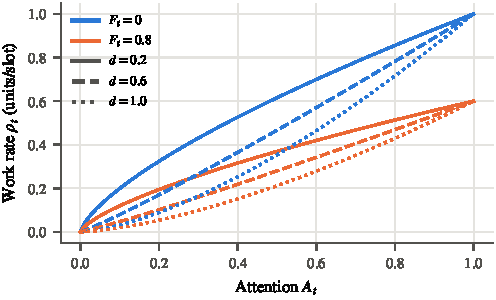
\includegraphics[width=0.55\textwidth]{figures/fig_efficiency.pdf}
\caption{Work rate as a function of attention for three difficulty levels and two fatigue levels.}
\label{fig:s-eff}
\end{figure}

\subsection{Environment variants used in the ablations}
\begin{itemize}
\item \textbf{No observation noise}: $\sigma_o=0$; the cognitive state is observed exactly (an MDP with respect to the cognitive variables, although future arrivals remain hidden).
\item \textbf{No circadian process}: $\gamma=0$, so that $A_t=H_t$.
\item \textbf{Static capacity (no cognition)}: $A_t\equiv0.60$ and $F_t\equiv0.30$ at all times. The resulting work rate of $0.60^{0.5+d}\times0.85$ (0.48 units/slot for $d=0.6$) delivers a daily throughput comparable to the break-taking heuristics in the full model, so the variant removes \emph{dynamics} without drastically changing \emph{capacity}. Breaks have no benefit in this variant.
\item \textbf{Task-only reward}: $\lambda=\mu=0$; the dynamics are unchanged.
\item \textbf{Worker profiles}: resilient ($\alpha,\delta\times0.7$; $\beta,\eta\times1.3$) and fatigue-prone ($\alpha,\delta\times1.3$; $\beta,\eta\times0.75$).
\item \textbf{Workload}: $N=8$ (4 initial) and $N=16$ (8 initial) tasks per day.
\end{itemize}

\section{Reproducibility}\label{sec:s-repro}
All experiments can be reproduced with the released code:
\begin{lstlisting}
pip install -r requirements.txt
python -m pytest                                 # simulator unit tests
python -m experiments.run_eval heuristics        # tune + test rule-based baselines
python -m experiments.run_rl --workers 4         # train all 107 agents
python -m experiments.run_eval robustness        # zero-shot robustness study
python -m experiments.run_eval traces            # behavioural traces
python -m analysis.analyze                       # all tables, figures, statistics
\end{lstlisting}
Seed ranges: training days $=s\times1\,000\,003+e$ for training seed $s$ and episode $e$; validation days $10^7,\dots,10^7+99$; test days $2\times10^7,\dots,2\times10^7+499$; tuning days $3\times10^7,\dots,3\times10^7+299$. One training run takes about \trainTimeAA{} s (AA-DQN) on a single CPU thread.
